\documentclass{article}
% Language setting
% Replace `english' with e.g. `spanish' to change the document language
\usepackage{biblatex} %Imports biblatex package
\addbibresource{sample.bib}
\usepackage{changepage}
\usepackage[english]{babel}
\usepackage{tikz}
\usepackage{array}
\usepackage{amsmath}
\usepackage{accents}
\usepackage{empheq}
\usepackage{pythonhighlight}
\newcolumntype{P}[1]{>{\centering\arraybackslash}p{#1}}
\newcolumntype{M}[1]{>{\centering\arraybackslash}m{#1}}

% Set page size and margins
% Replace `letterpaper' with `a4paper' for UK/EU standard size
\usepackage[letterpaper,top=2cm,bottom=2cm,left=3cm,right=3cm,marginparwidth=1.75cm]{geometry}

\usepackage{graphicx}
\usepackage[colorlinks=true, allcolors=blue]{hyperref}
\usepackage{setspace}
\usepackage{booktabs}
\usepackage[T1]{fontenc}
\usepackage{longtable}
\doublespacing

\begin{document}
\newcommand{\circled}[1]{\tikz[baseline=(char.base)]{
            \node[shape=circle,draw,inner sep=2pt] (char) {#1};}}

\newcommand{\pd}[3]{\frac{\partial^{#3}#1}{\partial {#2}^{#3}}}
\begin{titlepage}

\centering
\scshape
\vspace{\baselineskip}

%
\rule{\textwidth}{1.6pt}\vspace*{-\baselineskip}\vspace*{2pt}
\rule{\textwidth}{0.4pt}

{\Huge \textbf{\textsc{NPRE 449: Homework 9 \\
\vspace{15pt}}}}

\rule{\textwidth}{0.4pt}\vspace*{-\baselineskip}\vspace{3.2pt}
\rule{\textwidth}{1.6pt}\vspace{6pt}
%%\centerline{\textit{University of Illinois at Urbana-Champaign}} 
\vspace{1.5\baselineskip}


\large \centerline{\textbf{Author:} Nathan Glaser}
\large \centerline{\textbf{Net-ID:} nglaser3}
\quad

\vfill
\large \centerline{November 22, 2024}
%
\pagenumbering{gobble}
\end{titlepage}

\tableofcontents
\newpage
\pagenumbering{arabic}

\section{Derivation of Pin Temperature distribution}
First for the fuel. 
\begin{subequations}
    \begin{equation}
        \nabla k \nabla T_f + q''' = 0
    \end{equation}
    \begin{equation}
        \nabla^2T_f =\frac{1}{r}\pd{}{r}{}r\pd{T_f}{r}{}= - \frac{q'''}{k}
    \end{equation}
    \begin{equation}
        \pd{T_f}{r}{} = \frac{q''' r}{k_f} + C1\frac{1}{r}
    \end{equation}
    \begin{equation}
        T_f = \frac{q''' r^2}{4k_f} + C1\ln{r}+ C_2
    \end{equation}
\end{subequations}
Then for the gap.
\begin{subequations}
    \begin{equation}
        \nabla k \nabla T_g = 0
    \end{equation}
    \begin{equation}
        \pd{}{r}{}r\pd{T_g}{r}{} = 0
    \end{equation}
    \begin{equation}
        T_g = C_3\ln r + C_4
    \end{equation}
\end{subequations}
And finally for the clad.
\begin{subequations}
    \begin{equation}
        \nabla k \nabla T_c = 0
    \end{equation}
    \begin{equation}
        \pd{}{r}{}r\pd{T_c}{r}{} = 0
    \end{equation}
    \begin{equation}
        T_c = C_5\ln r + C_6
    \end{equation}
\end{subequations}

Next, our boundary conditions are:
\begin{itemize}
    \item[\circled{1}] $-k_f\nabla T_f (r = 0) = 0$
    \item[\circled{2}] $-k_f\nabla T_f(r=R_{f}) = -k_g\nabla T_g(r=R_{f})$
    \item[\circled{3}] $-k_g\nabla T_g(r=R_{c,i})=-k_c\nabla T_c(r=R_{c,i})$
    \item[\circled{4}] $T_c(r= R_{c,s}) = T_{c,s}$
    \item[\circled{5}] $T_g(r=R_{c,i}) = T_c(r=R_{c,i})$
    \item[\circled{6}] $T_f(r=R_f) = T_g(r=R_f)$
\end{itemize}

First, we can apply \circled{1}, also known as finiteness. This BC implies that $C_1$ is 0. Next, we investigate \circled{2}. Plugging in the respective temperature distributions, we get:
\begin{equation}
    \frac{q'''R_f}{2} = -\frac{k_gC_3}{R_f}
\end{equation}
Thus, we find $C_3$ to be:
\begin{equation}
    \boxed{C_3 = \frac{-q'''R_f^2}{2k_g}}
\end{equation}

Next, applying BC \circled{3}, and inserting the respective temperature distributions:
\begin{equation}
    -\frac{k_gC_3}{R_{c,i}} = -\frac{k_cC_5}{R_{c,i}}
\end{equation}
and thus, 
\begin{equation}
    \boxed{C_5 = \frac{k_g}{k_c}C_3}
\end{equation}

Proximally, applying \circled{4}, and solving for $C_6$, we obtain
\begin{equation}
    \boxed{C_6 = T_{c,s} - C_5\ln{R_{c,s}}}
\end{equation}

Next, investigating \circled{5}, rearranging for $C_4$,
\begin{equation}
    \boxed{C_4 = C_5\ln{R_{c,i}} + C_6 - C_3\ln(R_{c,i})}
\end{equation}

Then, finally we can determine $C_2$. Inserting all known parameters into \circled{6}, and rearranging, we get:
\begin{equation}
    \boxed{C_2 = C_3\ln(R_f) + C_4 + \frac{q'''R_f^2}{4k_f}}
\end{equation}

Now with all of our coefficients solved for, we just need to find $T_{c,s}$.
\section{Derivation of Fluid Temperature}
To begin, the area-averaged mass, momentum, and energy equations:
\begin{subequations}
    \begin{equation}
        \pd{\rho}{t}{} + \pd{\rho v}{z}{} = 0
        \label{mass}
    \end{equation}
    \begin{equation}
        \pd{\rho v}{t}{} + \pd{}{z}{}\rho v^2 = -\pd{P}{z}{}-\tau_F\frac{\xi_w}{A_f} - \rho g \sin(\theta)
        \label{momentum}
    \end{equation}
    \begin{equation}
        \pd{\rho h}{t}{} + \pd{}{z}{}\rho v h = \frac{q''\xi_h}{A}+\pd{P}{t}{} + q'''
        \label{energy}
    \end{equation}
\end{subequations}

First, looking at mass. This system is steady state, and $\rho v$ is also the mass-flux, G. Thus, the mass equation simplifies to:
\begin{equation}
    \pd{G}{z}{} = 0
\end{equation}

Next, the momentum equation is also steady-state, and again substituting in G for $\rho v$, we obtain
\begin{equation}
    -\pd{P}{z}{} = G^2\pd{}{z}{}\frac{1}{\rho} + \rho g + \tau_F\frac{\xi_w}{A_f}
\end{equation}
Then recognizing this as a potentially two-phase system, we substitute $\rho$ with $\rho_m$,
\begin{equation}
    -\pd{P}{z}{} = G^2\pd{}{z}{}\frac{1}{\rho_m} + \rho_m g + \frac{1}{2}f\frac{G^2\xi_w}{\rho_mA_f}
\end{equation}
such that
\begin{equation}
    \rho_m = \biggr[\frac{\chi}{\rho_g} + \frac{1-\chi}{\rho_f}\biggr]^{-1}
\end{equation}

Next, our energy equation. Again, steady state, $\rho_m v = G$, and also now no $q'''$ in the fluid.
\begin{equation}
    G\pd{}{z}{} h = \frac{q''\xi_h}{A}
\end{equation}

This is however not very helpful. Instead, we can write h in terms of the equilibrium quality, $X_e$. h in relation to $X_e$ is:
\begin{equation}
            h = h_{fg}\chi_e + h_{f,sat}
\end{equation}
Then the derivative of h is related to the derivative of $X_e$ by:
\begin{equation}
    \pd{h}{z}{} = \chi_e\pd{h_{fg,sat}}{z}{} + \pd{h_{f,sat}}{z}{} + h_{fg}\pd{\chi_e}{z}{}
\end{equation}
inserting this relation back into our energy equation, and solving for $\pd{\chi_e}{z}{}$, we obtain
\begin{equation}
    \pd{\chi_e}{z}{} = \frac{q''\xi_h}{A_fGh_{fg}} - \frac{1}{h_{fg}}\biggr[ \chi_e\pd{h_g}{z}{} + (1-\chi_e)\pd{h_f}{z}{}\biggr]
\end{equation}

now, because $\rho_m$ is dependent on $\chi$, we must expand the derivative of $\rho_m$ out with $\chi_e$. Substituting in $\biggr[\frac{\chi}{\rho_g} + \frac{1-\chi}{\rho_f}\biggr]^{-1}$ for $\rho_m$, then differentiating with respect to z, and substituting into our momentum equation:

\begin{equation}
    -\pd{P}{z}{} = \frac{\frac{1}{2}\frac{\xi_w}{A_f}f\frac{G^2}{\rho_m} + \rho_mg + \frac{GV_{fg}q''\xi_h}{A_fh_{fg}}}{1 - \frac{G^2V_{fg}}{h_{fg}}\biggr[ \chi_e\pd{h_g}{P}{} + (1-\chi_e)\pd{h_f}{P}{}\biggr]}
\end{equation}

Now with our general equations, we can solve with forward first-order finite  differencing. 

Approximating $\pd{A}{z}{}$ as $\frac{A^{i+1} - A^i}{\Delta z}$, we can solve for $A^{i+1}$ via simple rearranging.

Thus, our finite differencing equations:

\begin{subequations}
    \begin{equation}
        P^{i+1} = P^i - \Delta z \cdot \left[\frac{\frac{1}{2}\frac{\xi_w}{A_f}f\frac{G^2}{\rho_m} + \rho_mg + \frac{GV_{fg}q''\xi_h}{A_fh_{fg}}}{1 - \frac{G^2V_{fg}}{h_{fg}}\biggr[ \chi_e^i\pd{h_g}{P}{} + (1-\chi_e^i)\pd{h_f}{P}{}\biggr]}\right]
    \end{equation}
    \begin{equation}
        \chi_e^{i+1} = \chi_e^i + \Delta z \cdot \left[\frac{q''\xi_h}{A_fGh_{fg}} - \frac{1}{h_{fg}}\biggr[ \chi_e\pd{h_g}{z}{} + (1-\chi_e^i)\pd{h_f}{z}{}\biggr]\right]
    \end{equation}
\end{subequations}

\section{Clad Surface Temperature}
Now, with our fluid temperature we can solve for our wall temperature. 
Importantly, their are two regimes of heat transfer at the wall that we need to be aware of, $1\Phi$ and $2\Phi$. $1\Phi$ is simply newtons law of cooling, and thus the clad surface temp is trivial to solve for:
\begin{equation}
    T_{c,s} = \frac{q''}{h} + T_{fluid}
\end{equation}
However, in $2\Phi$ heat transfer, this hold another form:

\begin{subequations}
    \begin{equation}
        q'' = \biggr[\bigr[ Fh_{fc}(T_{c,s} - T_{fluid}) \bigr]^2 + \bigr[ S h_{nb}(T_{c,s} - T_{sat})\bigr]^2\biggr]^{1/2}
    \end{equation}
    \begin{equation}
        F = \biggr[ 1+ \chi Pr\left(\frac{\rho_f}{\rho_g} -1 \right)\biggr]^{-1}
    \end{equation}
    \begin{equation}
        S = \bigr[1+ 0.055F^{0.1}Re^{0.16}\bigr]^{-1}
    \end{equation}
    \begin{equation}
        h_{nb} = 55 \left(\frac{P}{P_c}\right)^{0.12}(q'')^{2/3}\left(\log\frac{P_c}{P}\right)M^{-1/2}
    \end{equation}
\end{subequations}
To find $T_{c,s}$ in $2\Phi$ heat transfer, the root of q'' needs to be found. Fortunately, this equation is non-transcendental and thus has 2 roots, but these roots are not guaranteed to be real, and positive. While this equation can be solved for $T_{c,s}$ analytically, root finding methods can also be employed. The function to find the root of is:
\begin{equation}
    q'' - \biggr[\bigr[ Fh_{fc}(T_{c,s} - T_{fluid}) \bigr]^2 + \bigr[ S h_{nb}(T_{c,s} - T_{sat})\bigr]^2\biggr]^{1/2} = 0
\end{equation}

This is done with \texttt{scipy.optimize.root}.

\newpage
\section{Figures}
First, the temperature plots. To begin, the fluid temperature, saturation temperature, the clad surface temperature, and the centerline temperature:
\begin{figure}[!hp!]
    \centering
    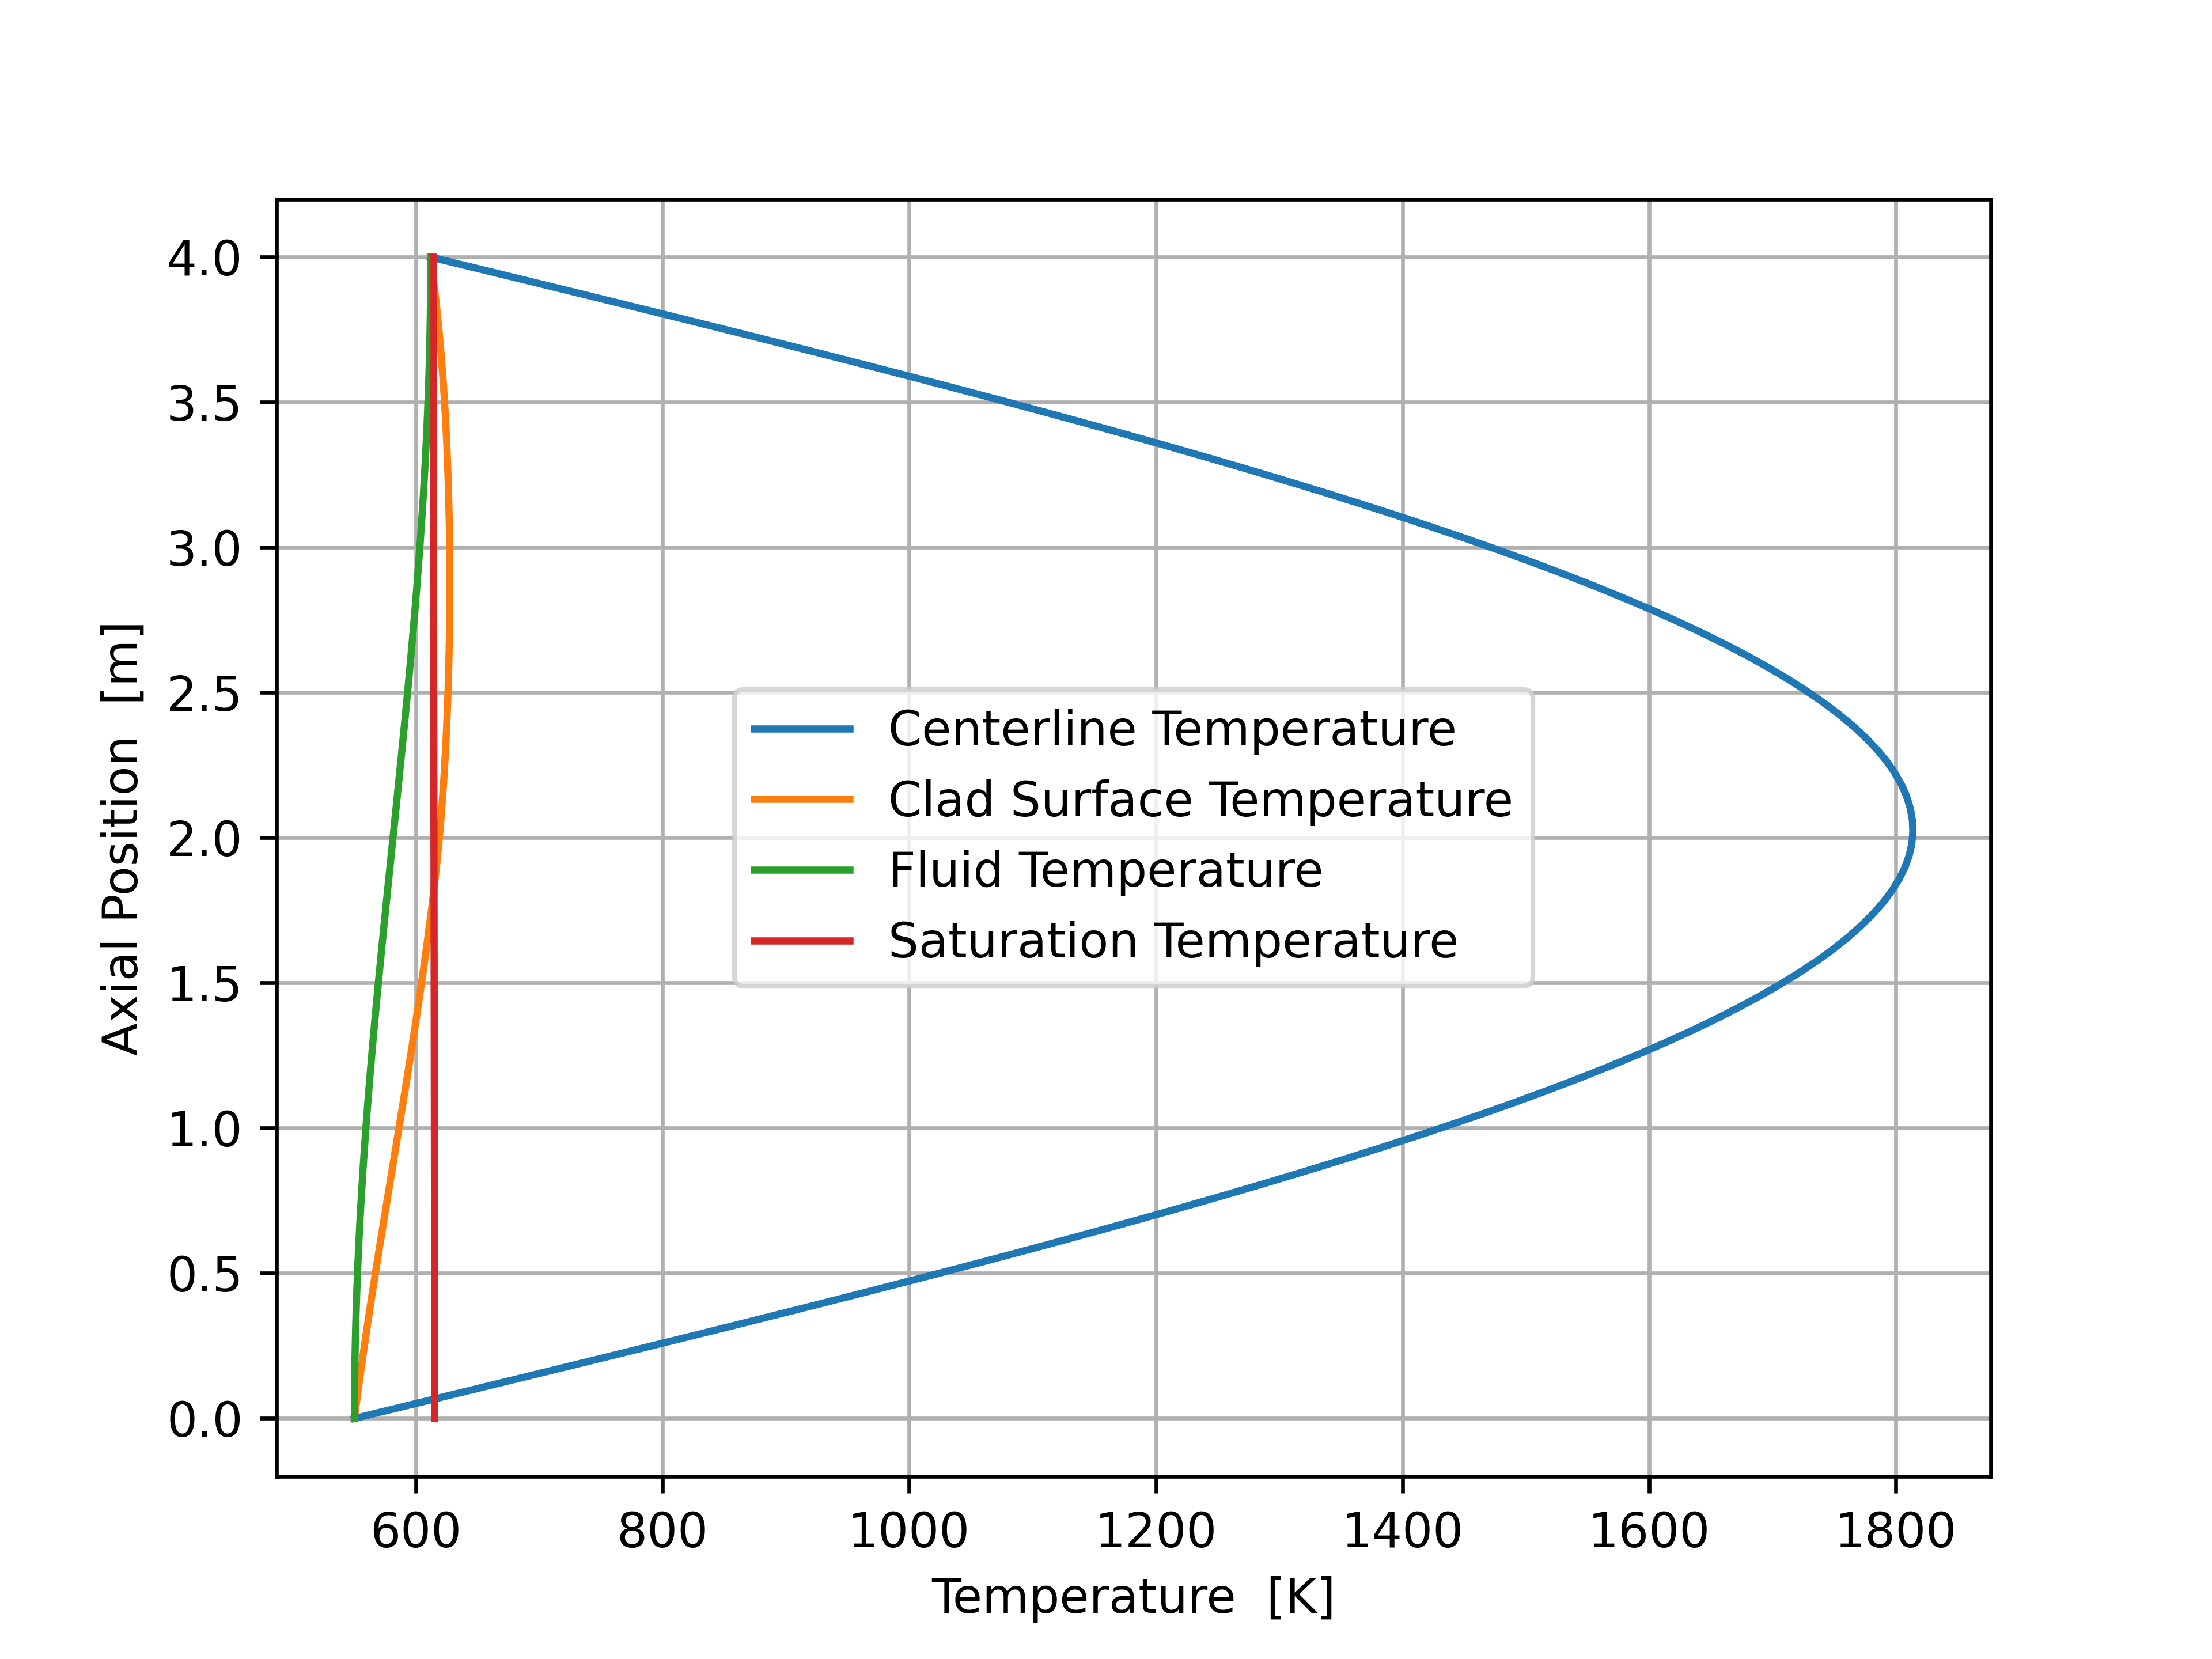
\includegraphics[width=0.5\linewidth]{tempplots.png}
\end{figure}

Then, zooming in on the non-centerline temperatures:
\begin{figure}[!hp!]
    \centering
    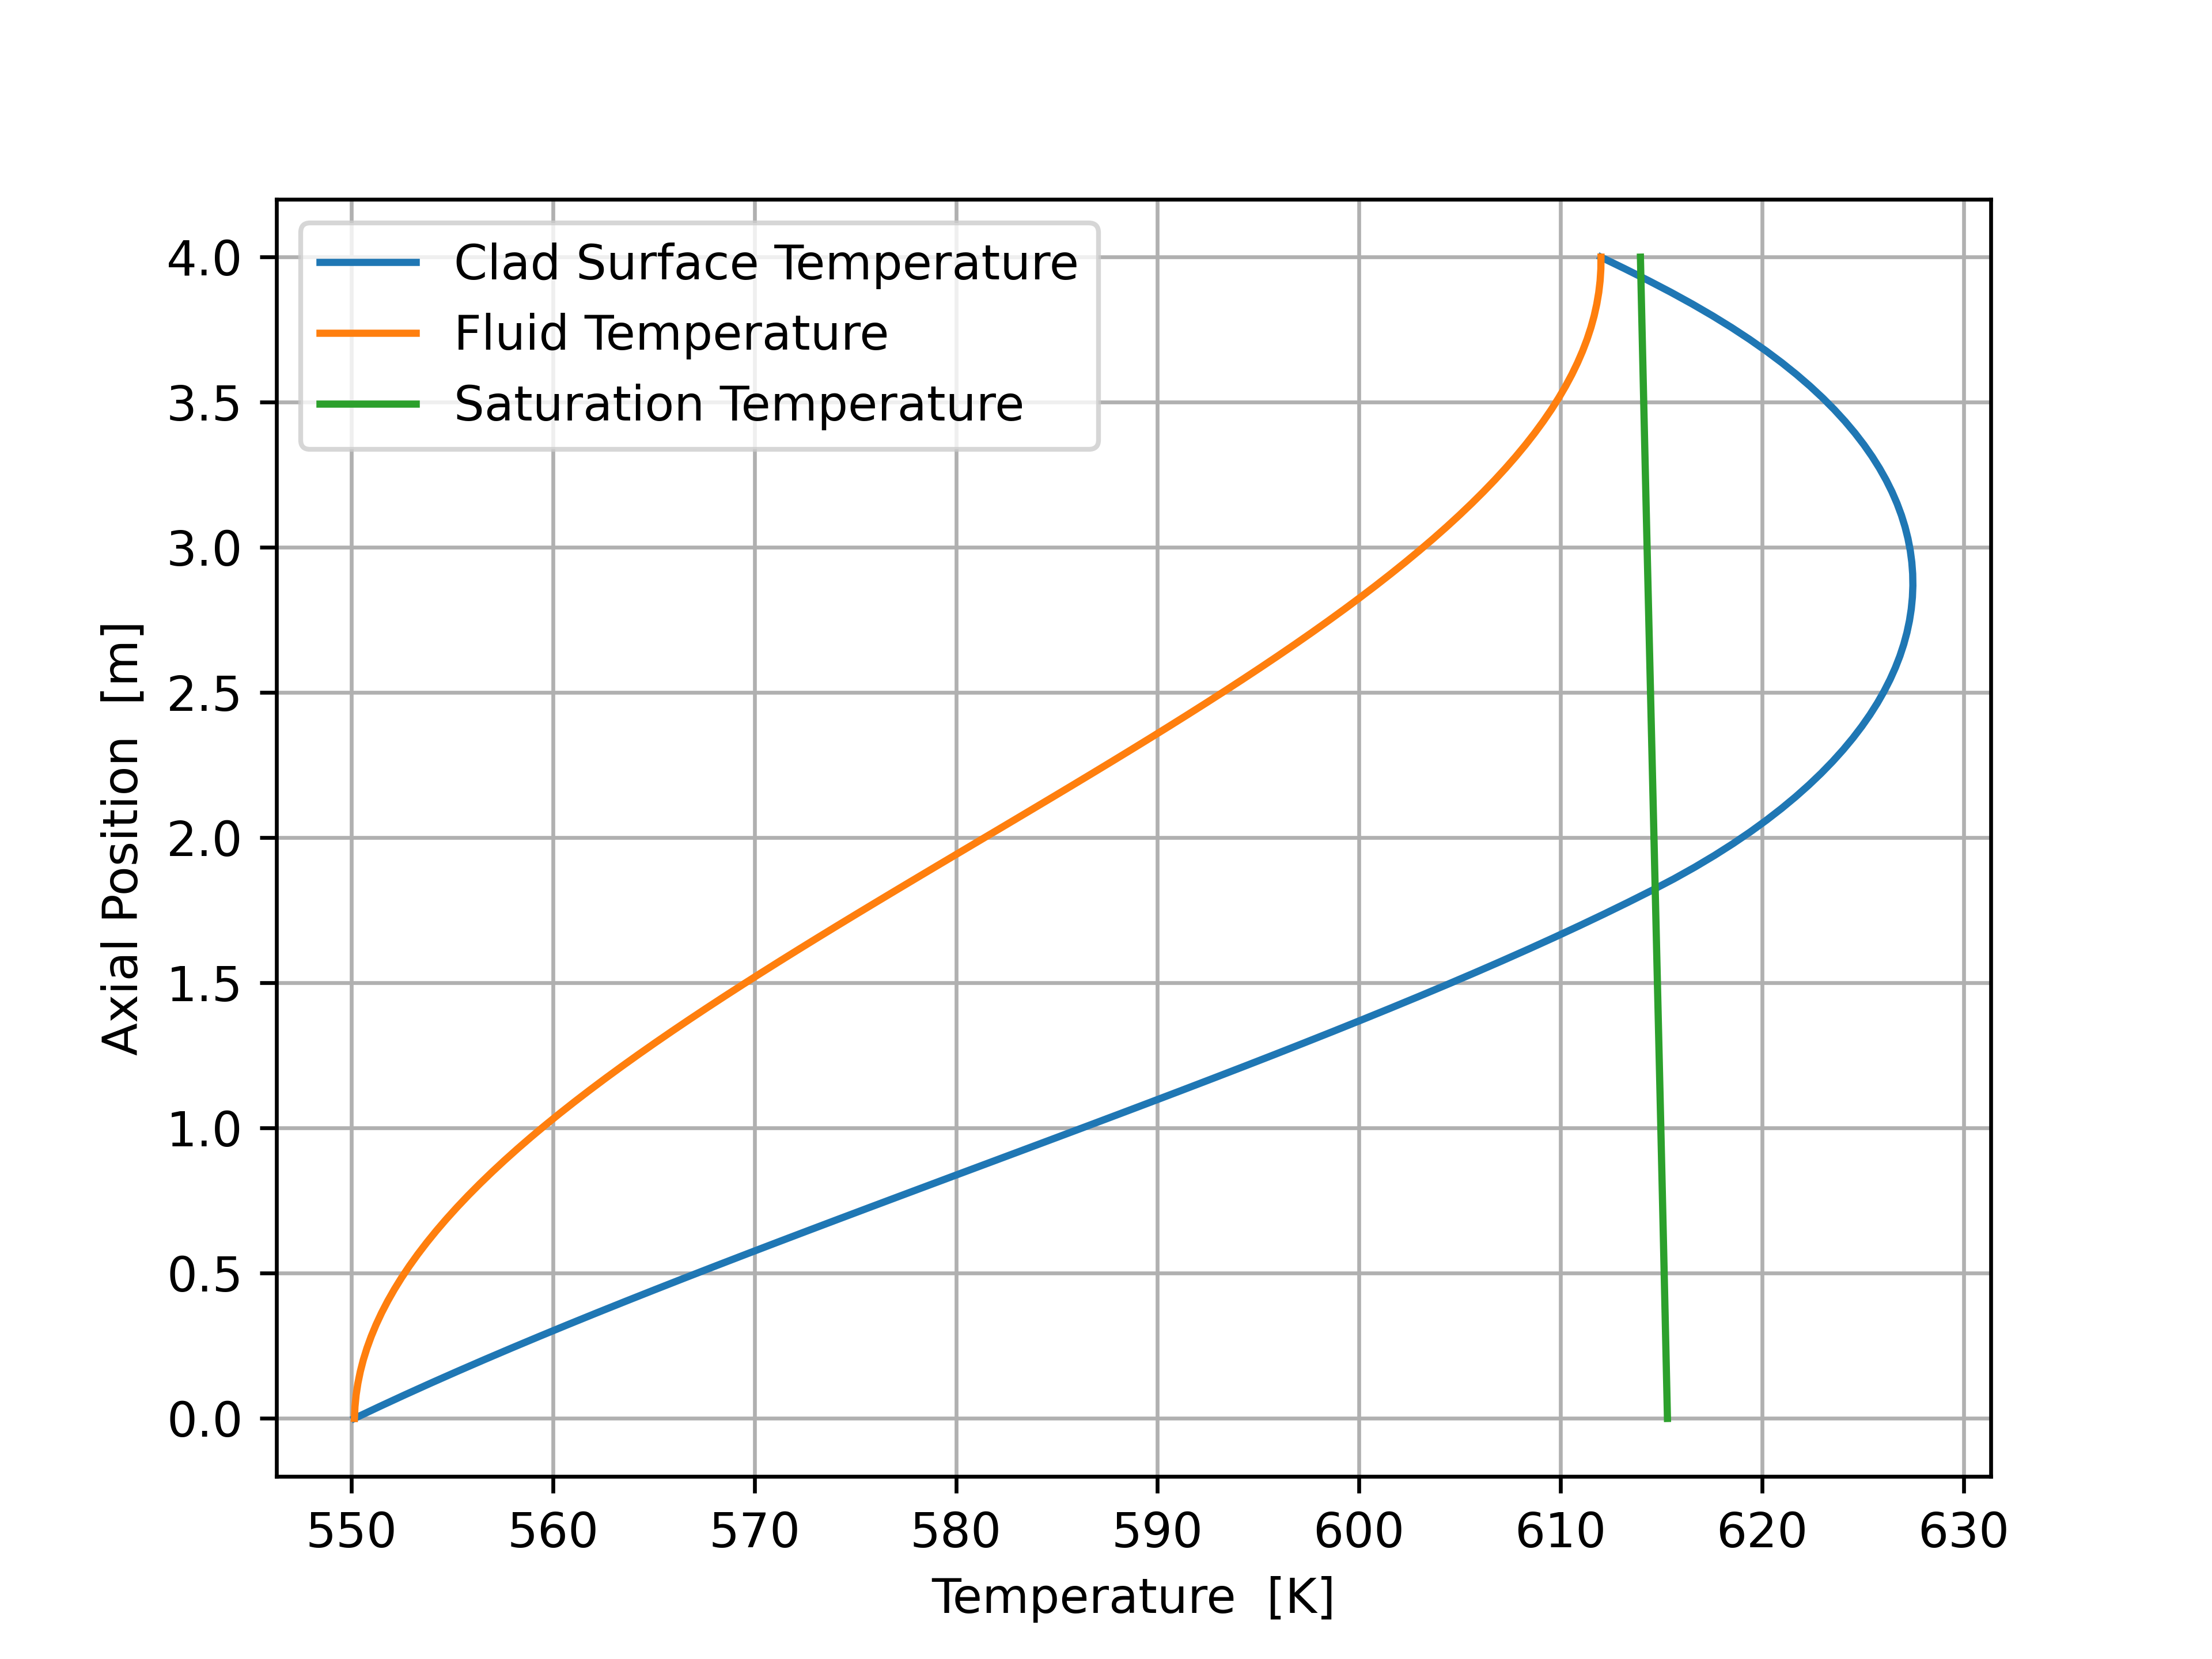
\includegraphics[width=0.5\linewidth]{tempnocl.png}
\end{figure}

\newpage
Next, the equilibrium quality:
\begin{figure}[!hp!]
    \centering
    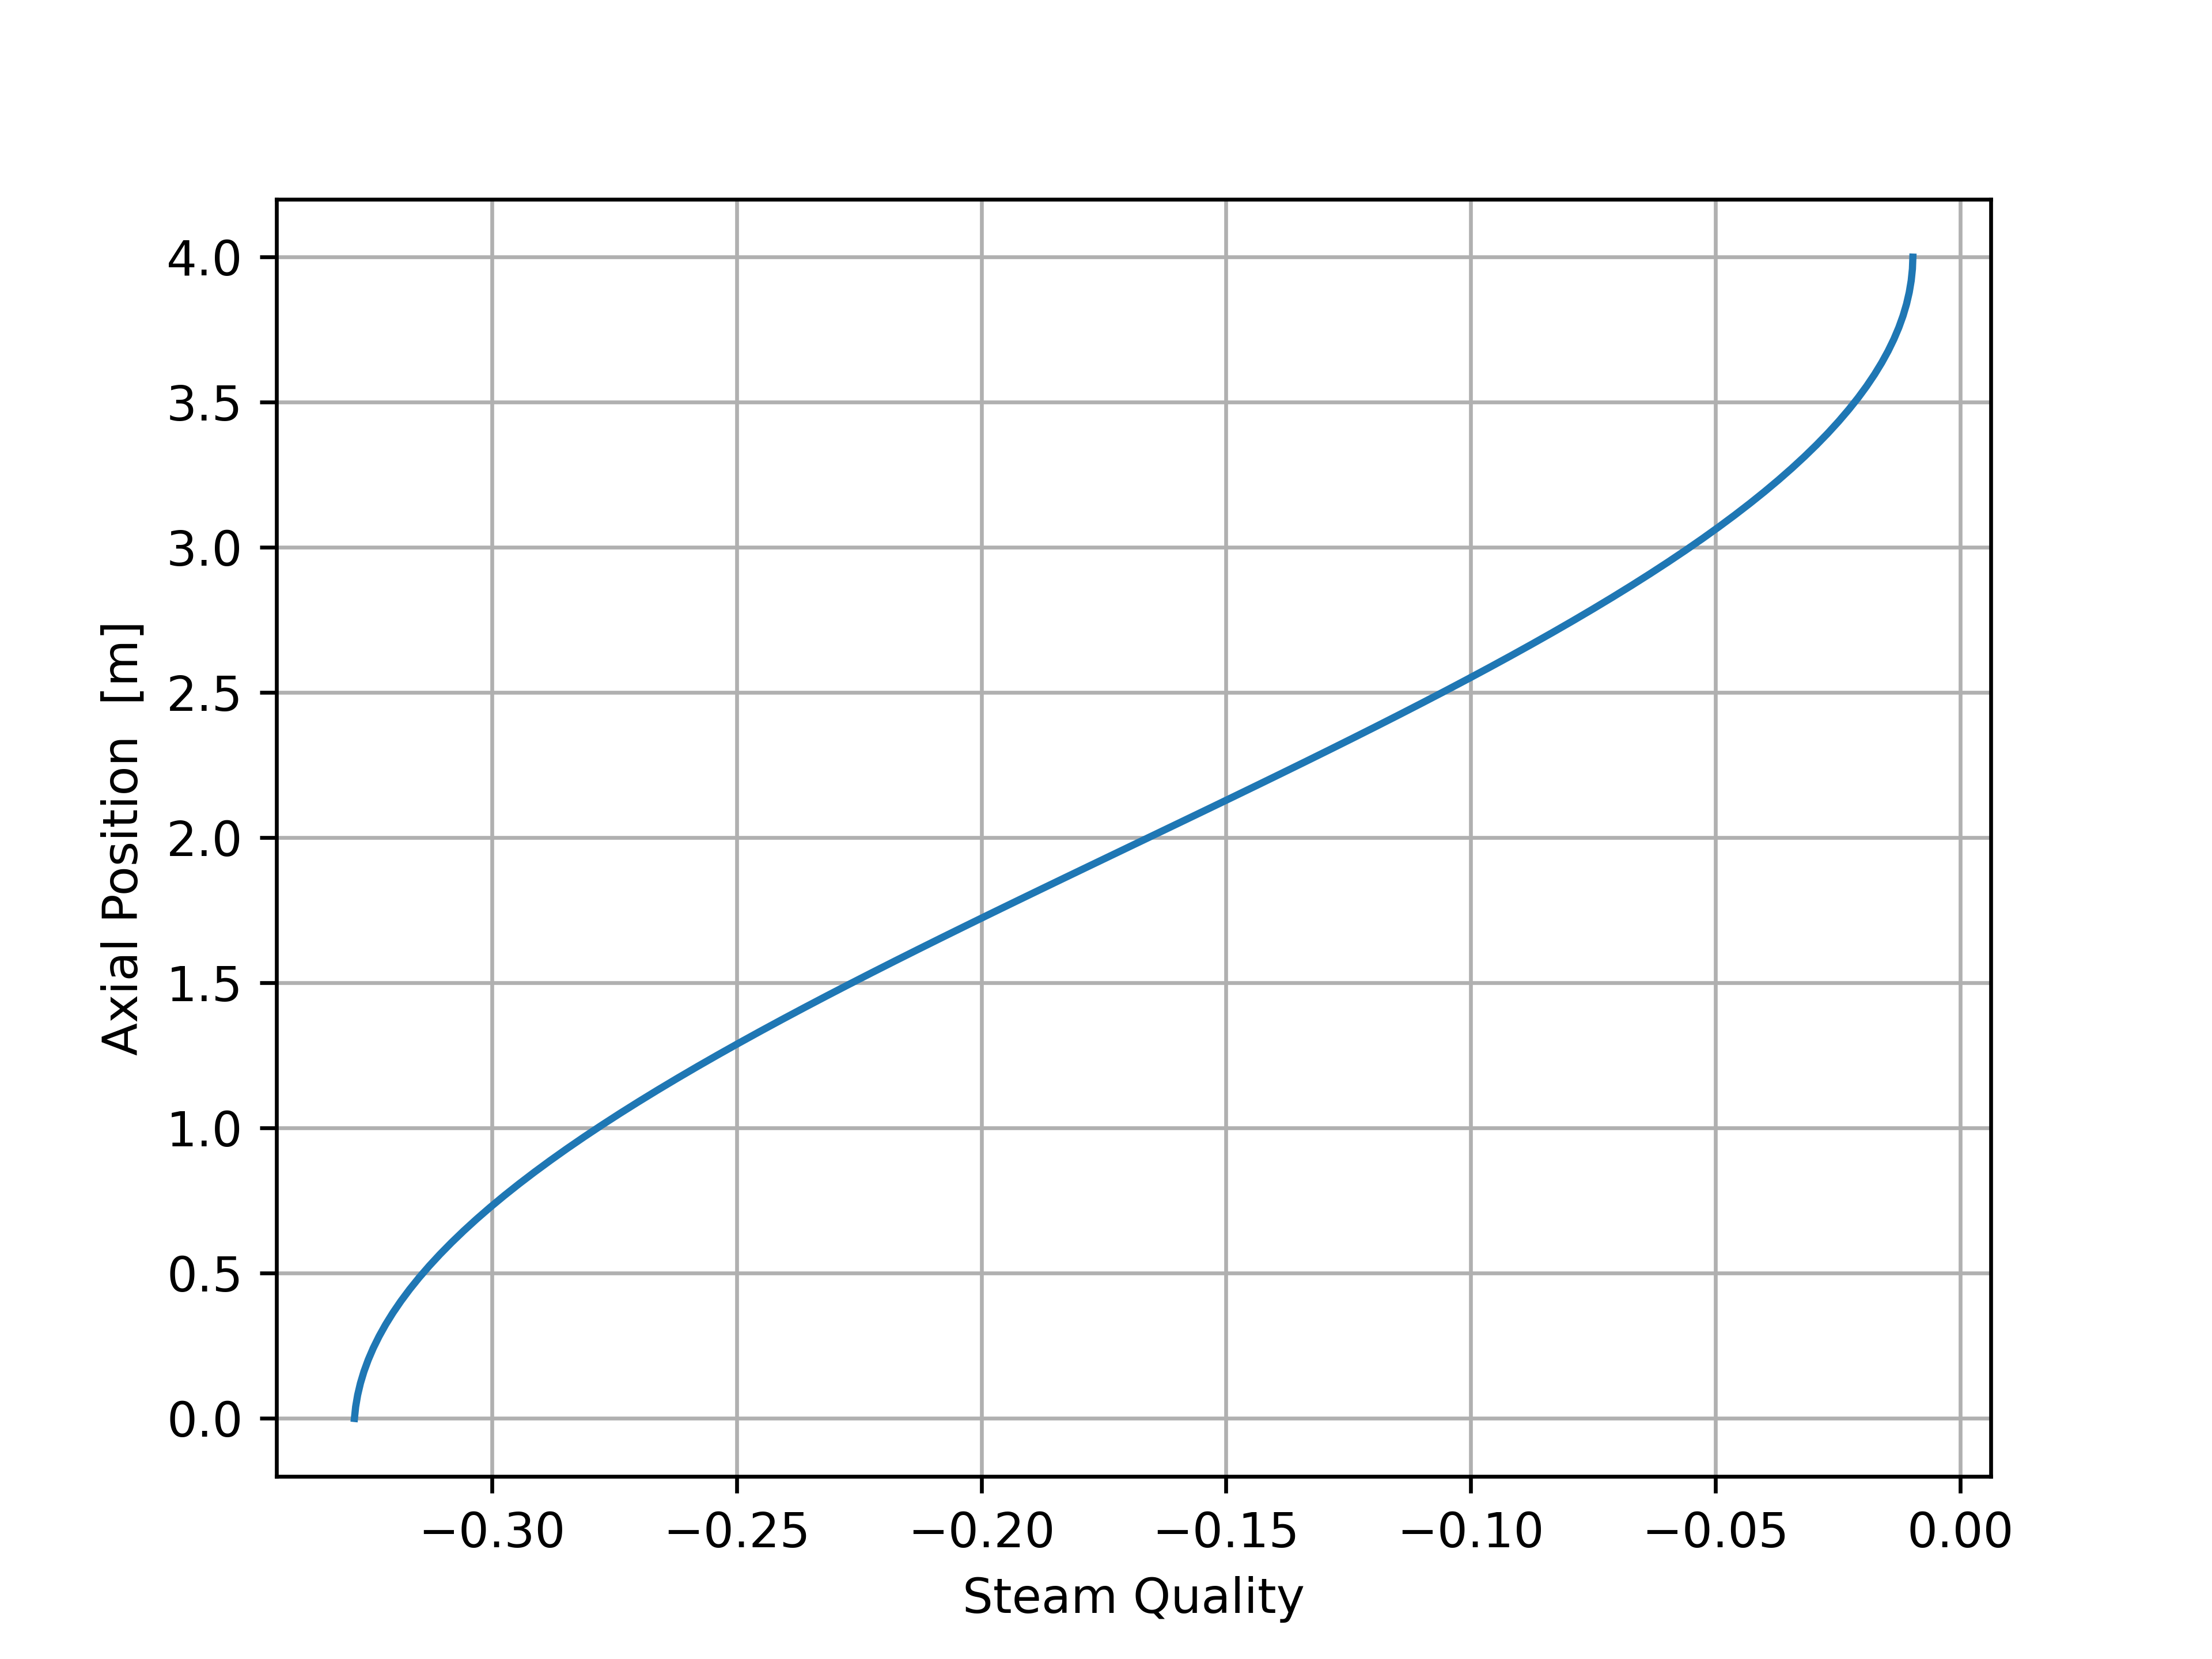
\includegraphics[width=0.5\linewidth]{xeplot.png}
\end{figure}

and finally the pressure:
\begin{figure}[!hp!]
    \centering
    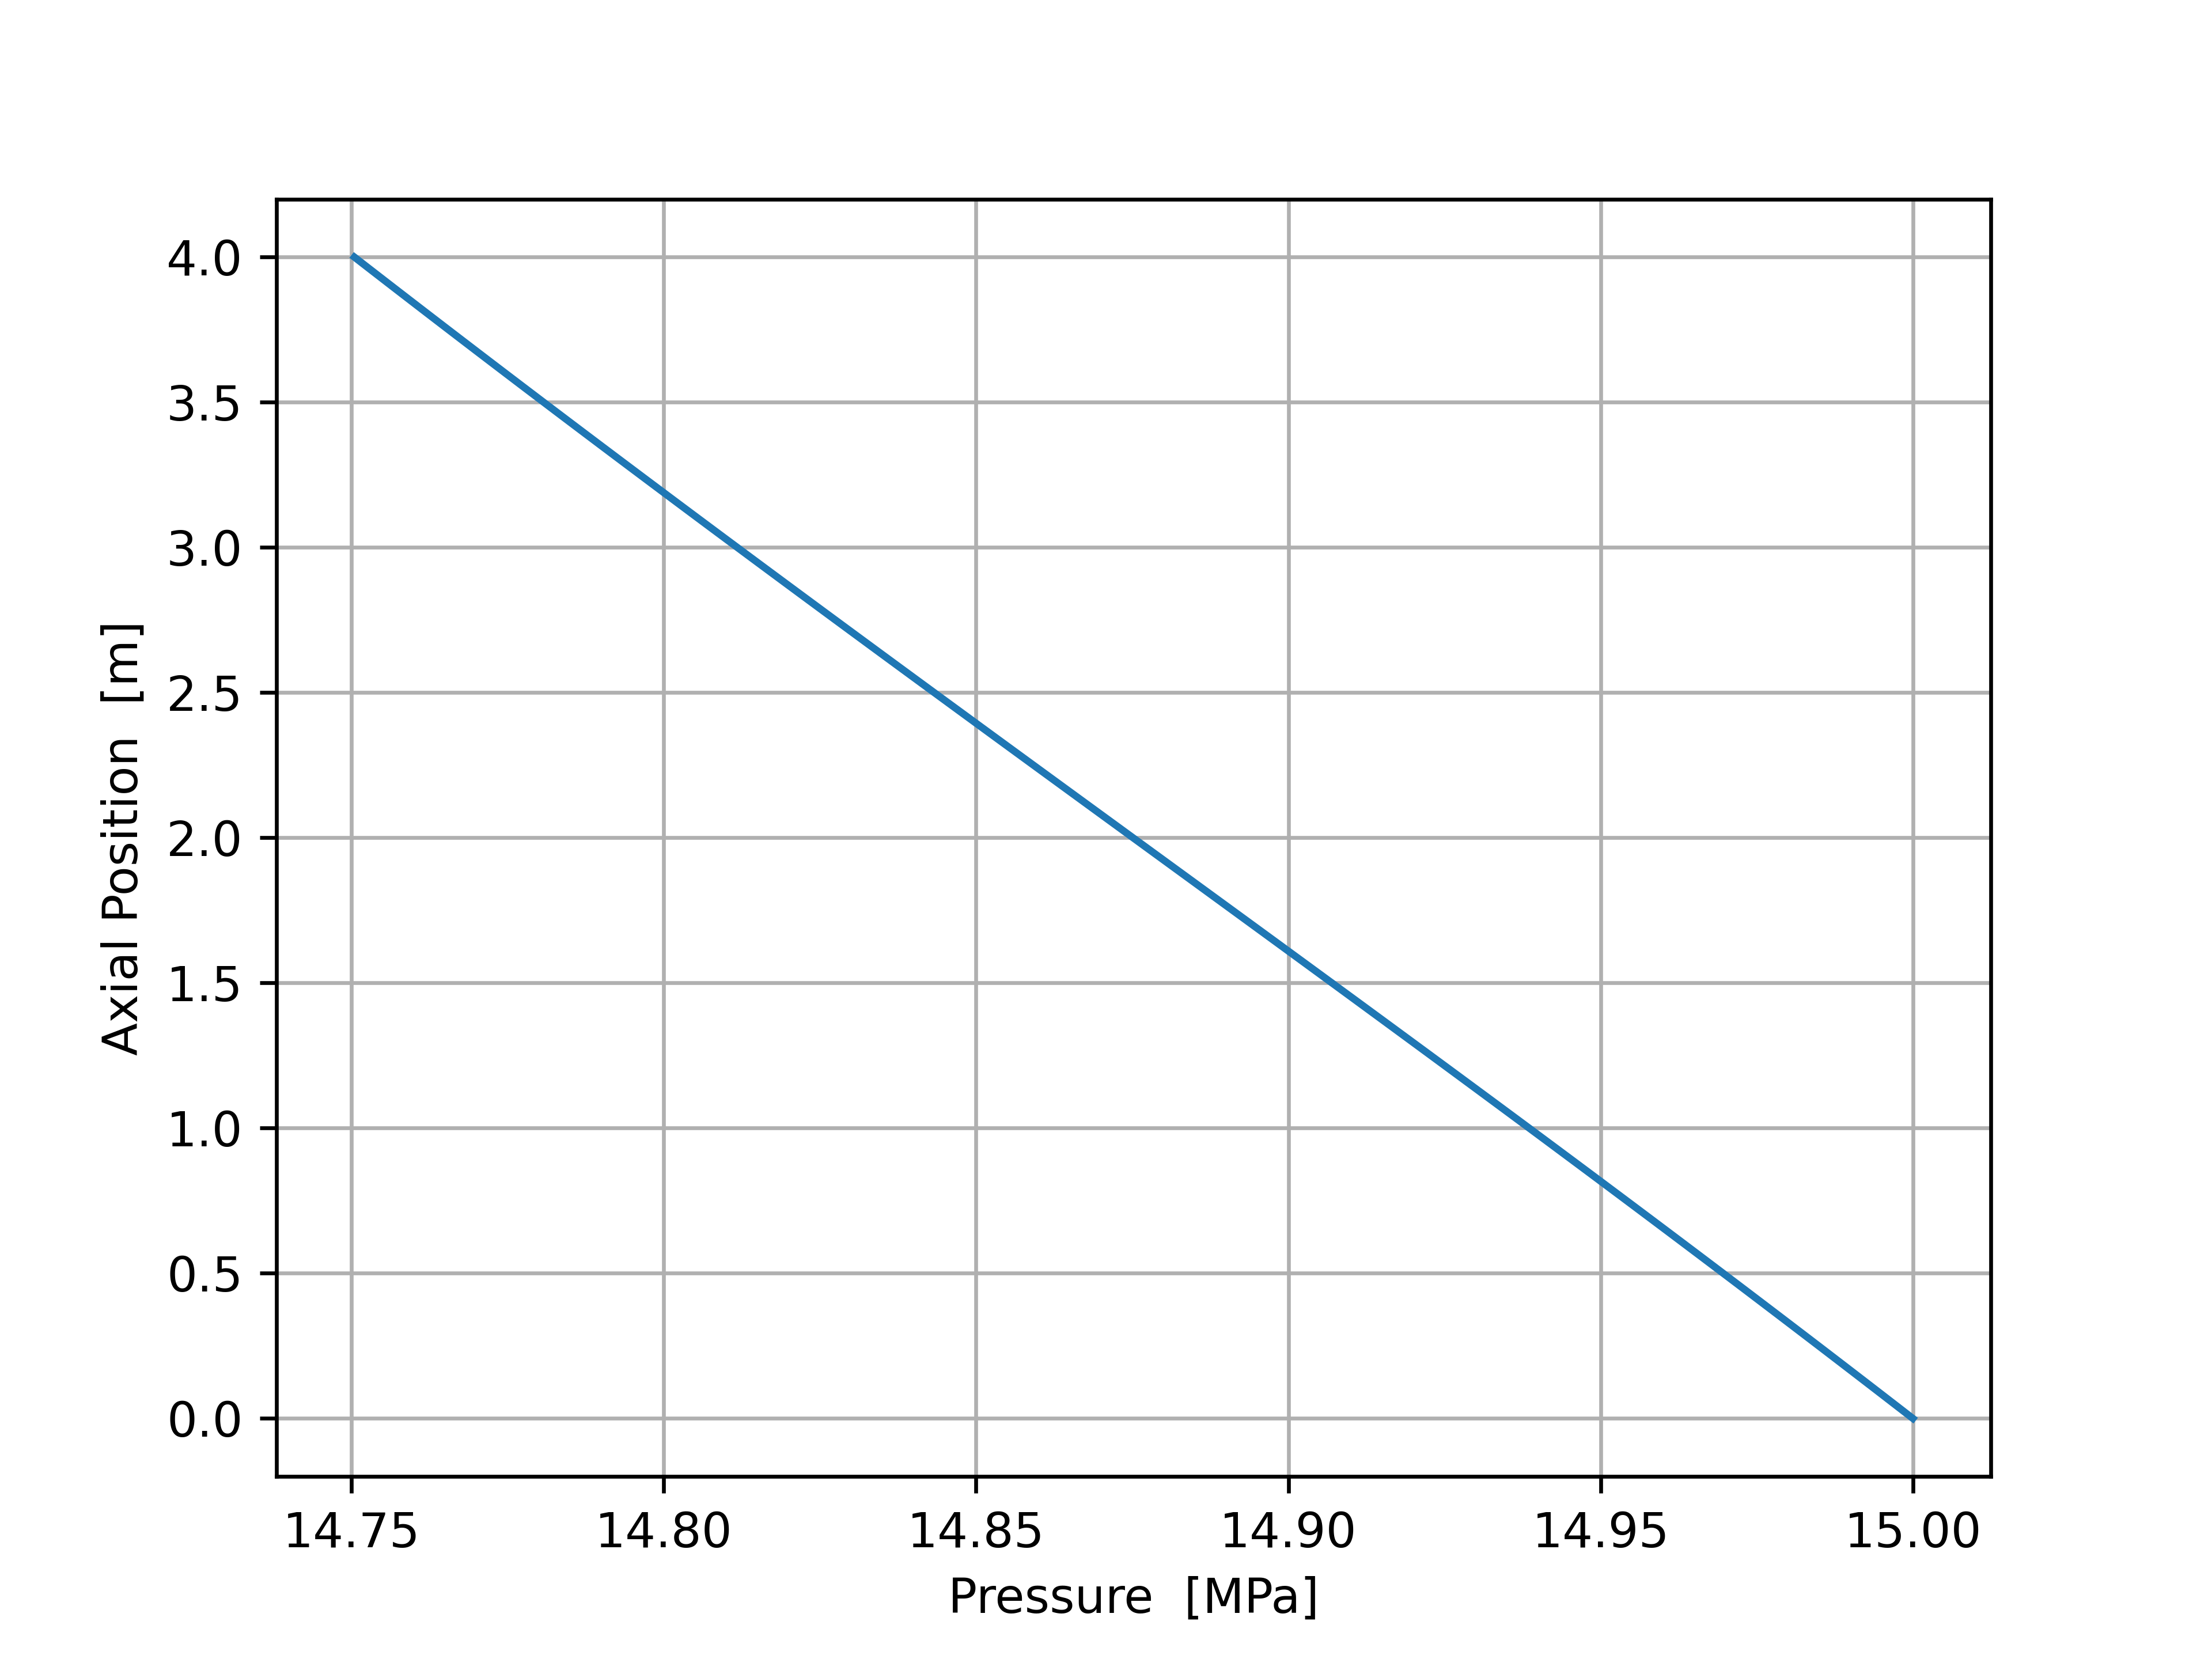
\includegraphics[width=0.5\linewidth]{pressureplot.png}
\end{figure}

\newpage
\section{Code Appendix}
\begin{python}
    import numpy as np
from numpy.linalg import norm as norm
import scipy as scp
import matplotlib.pyplot as plt
from pyXSteam.XSteam import XSteam
np.set_printoptions(precision=3,suppress= True)

class Conditions:
    
    def __init__(self,which = 'PWR'):
        
        self.g = 9.81 # m/s2
        
        if which == 'PWR':
            self.G = 4000 #kg/m2 s
            self.qp0 = 430e2 #W/cm to W/m
            self.P0 = 15e6 #MPa to pa
            self.Tf0c = 277 #oC
        
        else:
            self.G = 2350 #kg/m2 s
            self.qp0 = 605e2 #W/cm to W/m
            self.P0 = 7.5e6 #MPa to pa
            self.Tf0c = 272 #oC
            
        self.Tf0 = self.Tf0c + 273.15

class PinProperties:
    
    def __init__(self,Conditions,which = 'PWR'):
    
        if which == 'PWR':
            
            self.H = 4 #m
            self.Drod = 0.95e-2 # cm to m 
            self.Pitch = 1.26e-2 # cm to m
            self.DFuel = 0.82e-2 # cm to m
            self.Gap_thickness = 0.006e-2 #cm to m
            self.kgap=0.25 #W/mK
            self.k_fuel=3.6 #W/mK
            self.k_cladding=21.5 #W/mK
        
        else:
            
            self.H = 4.1 #m
            self.Drod = 1.227e-2 # cm to m
            self.Pitch = 1.62e-2 # cm to m 
            self.DFuel = 1.04e-2 # cm to m 
            self.Gap_thickness = 0.010e-2 # cm to m
            self.kgap=0.25 #W/mK
            self.k_fuel=3.6 #W/mK
            self.k_cladding=21.5 #W/mK

        
        self.xih = self.Drod * np.pi #m
        self.SAf = self.DFuel *np.pi * self.H
        self.SAc = (self.DFuel + self.Gap_thickness) * np.pi * self.H
        self.Axsf = self.DFuel ** 2 / 4 * np.pi
        self.Rf = self.DFuel/2
        self.Rci = self.Rf + self.Gap_thickness/2
        self.Rco = self.Drod / 2 
        self.qp = lambda z: Conditions.qp0* np.sin(np.pi * z / self.H) #W/m
        self.qpp = lambda z: self.qp(z) / self.xih # w /m2
        self.q3p = lambda z: self.qp(z) / self.Axsf
        
        return

class FluidProperties:
    
    def __init__(self,ICs,Pin,poly_order=15):
        
        '''
        Steam Table
        -----------
        '''
        props = XSteam(XSteam.UNIT_SYSTEM_BARE)
        
        '''
        Constant Material Properties 
        ----------------------------
        '''
        _p0,_tf0 = ICs.P0/1e6,ICs.Tf0 # Initial Pressure [MPa] and Temp [K]
        self.cp = props.Cp_pt(_p0,_tf0) * 1e3 #kj/kg -> j/kg
        self.mu = props.my_pt(_p0,_tf0)  # N s / m2
        self.k = props.tc_pt(_p0,_tf0)  # W/ m K

        '''
        Pressure Variant Properties
        ---------------------------
        '''
        self.hg = lambda P: props.hV_p(P) * 1e3 # kJ/kg -> j/kg
        self.hf = lambda P: props.hL_p(P) * 1e3 # kJ/kg -> j/kg
        self.hfg = lambda P: self.hg(P) - self.hf(P)
        self.tsat = lambda P: props.tsat_p(P) # K

        '''
        Initial Properties
        ------------------
        '''
        self.X_e0 = self.cp*(_tf0 - self.tsat(_p0))/self.hfg(_p0)
        self.rho0 = props.rho_pt(_p0,_tf0) #kg /m3

        '''
        Pipe Dimensions
        ---------------
        '''
        self.Area = (Pin.Pitch**2 - 1/4 * np.pi * Pin.Drod**2) #m2
        self.xiw = Pin.xih #m
        self.Dh = 4 * self.Area / (self.xiw) #m
        
        '''
        Dimensionless Groups +
        ----------------------
        '''
        self.Re = ICs.G * self.Dh / self.mu
        self.Pr = self.cp * self.mu / self.k
        self.Nu = 0.023 * self.Re**(.8) * self.Pr ** (0.4)
        self.h = self.Nu * self.k / self.Dh 
        self.__f = self.Re ** (-.25) * 0.316

        '''
        Two-Phase Properties
        --------------------
        '''
        self.rhosatratio = lambda P: props.rhoV_p(P) / props.rhoL_p(P)
        self.alpha = lambda Xe: 1 / (1 + (Xe**(-1) - 1) * self.rhosatratio(_p0))
        self.rhofg = props.rhoL_p(_p0) - props.rhoV_p(_p0)
        self.rhoL = props.rhoL_p(_p0)
        self.rhoV = props.rhoV_p(_p0)
        self.rhom = lambda Xe, P: self.rhoL if Xe<0 else (1/self.rhoL + 1/self.rhofg*Xe)**(-1)
            #for props.my_pt, for whatever reason pyXSteam doesnt have mu at saturation
            #so you have to alter tsat a littlebit
        self.muL = lambda P: props.my_ph(P, props.hL_p(P))
        self.__muV = lambda P: props.my_ph(P, props.hV_p(P))
        self.mum = lambda Xe, P: self.mu if Xe <0 else (Xe / self.__muV(P) + (1 - Xe)/self.muL(P))**(-1)
        self.f = lambda Xe, P: self.__f if Xe <0 else self.__f* (self.mum(Xe, P) / self.muL(P))


        '''
        Material Property Fits
        ----------------------
        '''
        self.__pressures = np.linspace(1,20,1000)
        self.__hf_data = [self.hf(P) for P in self.__pressures] 
        self.__hg_data = [self.hg(P) for P in self.__pressures]

        #fitting with 15th order polynomial with numpy.polyfit and np.polynomial.Polynomials
        #polyfit returns high -> low, polynomial.Polynomial takes low -> high 
        #only setting as object for plotting
        self.__hf_fit = np.polynomial.Polynomial( np.flip( np.polyfit(self.__pressures*1e6,self.__hf_data,poly_order) ) ) 
        self.__hg_fit = np.polynomial.Polynomial( np.flip( np.polyfit(self.__pressures*1e6,self.__hg_data,poly_order) ) ) 

        self.dhfdp = self.__hf_fit.deriv()
        self.dhgdp = self.__hg_fit.deriv()
        
        return

    def plot(self):
        
        p,hfdata,hgdata = self.__pressures, self.__hf_data, self.__hg_data
        hf_fit = self.__hf_fit(p*1e6)
        hg_fit = self.__hg_fit(p*1e6)

        hf_norm = norm(hf_fit - hfdata,2) / norm(hfdata,2)
        hg_norm = norm(hg_fit - hgdata,2) / norm(hgdata,2)
        
        fig,ax = plt.subplot_mosaic([['h_f','h_g']],figsize = (12,5),gridspec_kw={'wspace':.2})
        
        ax['h_f'].plot(p, hfdata, label = 'pyXSteam Data')
        ax['h_f'].plot(p, hf_fit, label = 'h$_f$ Polynomial Fit')
        ax['h_f'].set_ylabel('h$_f$  [J $\cdot$ kg$^{-1}$]')

        ax['h_g'].plot(p, hgdata, label = 'pyXSteam Data')
        ax['h_g'].plot(p, hg_fit, label= 'h$_{g}$ Polynomial Fit')
        ax['h_g'].set_ylabel('h$_{g}$  [J $\cdot$ kg$^{-1}$]')

        for plot in ax:
            ax[plot].set_xlabel('Pressure  [MPa]')
            ax[plot].grid()
            ax[plot].legend()

        print(f'hf Fit L2 Norm: {hf_norm}\nhg Fit L2 Norm: {hg_norm}')
        
        
        return 
        
'''
SOLVER
'''
class Solver:
    
    def __init__(self,which = 'PWR',num_zsteps = 100):
        try:
            assert(which in ['PWR','BWR'])
        except AssertionError:
            errormessage = f"The reactor type '{which}' is not supported. Valid reactor types are: 'BWR' or 'PWR'"
            raise Exception(errormessage)
        self.which = which
        self.ICs = Conditions(which=which)
        self.pin = PinProperties(which=which,Conditions=self.ICs)
        self.fluid = FluidProperties(self.ICs,self.pin)
        self.z = np.linspace(0,self.pin.H,num_zsteps)
        
        return


    def solveFluid(self,output = True):
        
        ICs,pin, fluid = self.ICs, self.pin, self.fluid
        z = self.z
        P = [ICs.P0]
        X_e = [fluid.X_e0]
        T_f = [ICs.Tf0]
        if output:
            print('Z-Coordinate\tPressure\tSteam Quality\tFluid Temperature')
            print('-----------------------------------------------------------------')
            print(f'{np.trunc(z[0],)}\t\t{np.around(P[0]*1e-6,3)}\t\t{np.around(X_e[0],4)}\t\t{np.around(T_f[0],3)}')
        for i in range(1, len(z)):
            
            dz = z[i]- z[i-1]
            
            '''
            Solving for Pressure
            Solve for pressure using the material properties at the previous z
            '''
            rhom = fluid.rhom(X_e[i-1],P[i-1]*1e-6)
            topP1 = 1/2 * fluid.xiw / fluid.Area * fluid.f(X_e[i-1],P[i-1]*1e-6) * ICs.G**2 / rhom
            topP2 = rhom * ICs.g
            topP3 = ICs.G * pin.qp(z[i]) / (fluid.rhofg * fluid.Area * fluid.hfg(P[i-1]*1e-6))
            botP1 =  fluid.dhfdp(P[i-1]) if X_e[i-1] < 0 else X_e[i-1] * fluid.dhgdp(P[i-1]) + (1-X_e[i-1]) * fluid.dhfdp(P[i-1])
            botP2 = 1 - ICs.G**2 / (fluid.rhofg * fluid.hfg(P[i-1]*1e-6)) * botP1
            insideP = (topP1 + topP2 + topP3) / botP2
            P_i = P[i-1] - dz *insideP

            '''
            Solving for Steam Quality
            Solve for steam quality using current pressure
            '''
            dpdz = (P_i - P[i-1]) / dz
            insideXe1 = fluid.dhfdp(P_i) * dpdz if X_e[i-1] < 0 else X_e[i-1] * fluid.dhgdp(P_i) * dpdz + (1 - X_e[i-1]) * fluid.dhfdp(P_i) * dpdz
            insideXe2 = pin.qp(z[i]) / (fluid.Area * ICs.G * fluid.hfg(P_i* 1e-6)) - 1/fluid.hfg(P_i * 1e-6) * insideXe1
            X_e_i = dz * insideXe2 + X_e[i-1]

            '''
            Solving for Temperature
            Find temperature with current properties
            '''
            T_f_i = fluid.hfg(P_i*1e-6) / fluid.cp * X_e_i + fluid.tsat(P_i*1e-6) if X_e_i < 0 else fluid.tsat(P_i*1e-6)

            '''
            Printing
            '''
            if output:
                print(f'{np.around(z[i],3)}\t\t{np.around(P_i*1e-6,3)}\t\t{np.around(X_e_i,4)}\t\t{np.around(T_f_i,3)}')
            
            '''
            Appending Pressure, Steam Quality, and Fluid Temperature lists
            lists are better than numpy arrays for on the fly changing...
            '''
            P.append(P_i)
            X_e.append(X_e_i)
            T_f.append(T_f_i)
            
        
        self.PFunc = scp.interpolate.interp1d(z,np.array(P)*1e-6)
        self.XeFunc = scp.interpolate.interp1d(z,X_e)
        self.TFluidFunc = scp.interpolate.interp1d(z,T_f)
        
        return


    def __solveCladSurface(self):

        ICs,pin, fluid = self.ICs, self.pin, self.fluid

        Pc = 22.06
        M = 18.01528
        F = lambda Xe,P: 1 if Xe < 0 else (1 + Xe * fluid.Pr * (fluid.rhosatratio(P) - 1)) ** (0.35)
        S = lambda Xe,z: (1 + 0.055 * F(Xe,self.PFunc(z)) ** (0.1) * (ICs.G * fluid.Dh / fluid.muL(ICs.P0/1e6))**(0.16)) ** (-1)
        hnb = lambda z: 55 * (self.PFunc(z) / Pc) ** (0.12) * pin.qpp(z)**(2/3) * (-np.log(self.PFunc(z)/Pc)) * M**(-0.5)
        def twophase(Tw,z,Xe):
            fpart = (F(Xe,self.PFunc(z)) * fluid.h * (Tw - self.TFluidFunc(z)))**2
            spart = (S(Xe,z) * hnb(z) *(Tw - fluid.tsat(self.PFunc(z))))**2
            return pin.qpp(z) - (fpart + spart) **(.5)
        def onephase(z):
            return pin.qpp(z) / fluid.h + self.TFluidFunc(z)

        T_cs = []
        guess = fluid.tsat(ICs.P0/1e6) *1.5
        for i,z in enumerate(self.z):
            X_e_i = self.XeFunc(z)
            tempGuess = onephase(z)
            if tempGuess < fluid.tsat(self.PFunc(z)):
                T_cs.append(tempGuess)
            else:
                try:
                    _ = self.ONB * 3
                except:
                    self.ONB = z
                func = lambda Tw: twophase(Tw,z,X_e_i)
                root = scp.optimize.root(func,guess).x[0]
                T_cs.append(root)

        try:
            self.SatBoil = scp.optimize.root(self.XeFunc, pin.H/3).x[0]
        except ValueError:
            pass
        self.TCladS = scp.interpolate.interp1d(self.z,T_cs)
        return
            

    def solvePinTemperature(self):

        self.__solveCladSurface()
        ICs,pin, fluid = self.ICs, self.pin, self.fluid

        C3 = lambda z: -pin.q3p(z)*pin.Rf**2 / 2 / pin.kgap #yes
        C5 = lambda z: pin.kgap / pin.k_cladding * C3(z) 
        C6 = lambda z: self.TCladS(z) - C5(z)*np.log(pin.Rco)
        C4 = lambda z: C5(z)* np.log(pin.Rci) - C3(z)* np.log(pin.Rci) + C6(z)
        C2 = lambda z: pin.q3p(z) * pin.Rf**2 / 4 / pin.k_fuel + C3(z) * np.log(pin.Rf) + C4(z)

        self.TFuelFunc = lambda r, z: -pin.q3p(z) * r**2 / 4 / pin.k_fuel + C2(z)
        self.TGapFunc = lambda r, z: C3(z) * np.log(r) + C4(z)
        self.TCladFunc = lambda r, z: C5(z) * np.log(r) + C6(z)
        
        return
        

class Plotter:
    
    def __init__(self, which = 'PWR', ideal_steps = 1000, show = False):

        self.zsteps = ideal_steps
        solver = Solver(which=which,num_zsteps=self.zsteps)
        solver.solveFluid(output=False)
        solver.solvePinTemperature()
        self.solution = solver
        try:
            assert(which in ['PWR','BWR'])
        except AssertionError:
            errormessage = f"The reactor type '{which}' is not supported. Valid reactor types are: 'BWR' or 'PWR'"
            raise Exception(errormessage)
        self.__MESH(which,show)
        self.__BOTH(show)
        if which == 'BWR':
            self.__BWR(show)
        self.__SENSITIVITY(which)
        return
    def __finisher(self, ax, xlabel='t',legend=0,loc=None):
        xlabel = 'Temperature  [K]' if xlabel == 't' else 'Pressure  [MPa]'
        ax.grid()
        if legend:
            ax.legend(loc = loc)
        ax.set_xlabel(xlabel)
        ax.set_ylabel('Axial Position  [m]')
    def __radfinisher(self, ax):
        ax.grid()
        ax.legend()
        ax.set_xlabel('Radial Position  [m]')
        ax.set_ylabel('Temperature  [K]')

    @staticmethod
    def __show(show):
        if show:
            plt.show()
        else:
            plt.close()
        
    @staticmethod   
    def __latex(arr, name):
        component = f'{name} & '
        maxcl = 'T_{max,CL}  [$K$] & '
        for comp, tcl in arr:
            component += str(comp) + ' & '
            maxcl += str(np.around(tcl,3)) + ' & '

        print('\\toprule\n\\bottomrule')
        print(component[:-2]+'\\\\')
        print('\hline')
        print(maxcl[:-2]+'\\\\')
        
        return


    def __MESH(self, which,show =False):
        fig, ax = plt.subplots()
        for n in [2,3,5,10,100, 1000]:
            solve = Solver(which,n)
            solve.solveFluid(output=False)
            ax.plot(solve.TFluidFunc(solve.z), solve.z, label = f'{n} Nodes')
        self.__finisher(ax,legend=1)
        self.__show(show)
        return

    def __BOTH(self, show = False):

        solution = self.solution
        z = solution.z

        TFluid = solution.TFluidFunc(z)
        TCladSO = solution.TCladS(z)
        TCladSI = solution.TCladFunc(solution.pin.Rci,z)
        TFuelS = solution.TFuelFunc(solution.pin.Rf,z)
        TFuelCL = solution.TFuelFunc(0,z)

        print('\tMaximum Temperatures')
        print('------------------------------------')
        print(f'Fuel: {max(TFuelCL)}\nClad: {max(TCladSI)}\nFluid: {max(TFluid)}')
        zmaxCL = z[np.where(TFuelCL == max(TFuelCL))[0][0]]
        Pressure = solution.PFunc(z)
        TSat = [solution.fluid.tsat(p) for p in Pressure]

        '''Temperatures'''
        fig, ax = plt.subplots()
        ax.plot(TFluid,z, label = 'Fluid Temperature')
        ax.plot(TSat, z, label = 'Saturation Temperature', color = 'k', linestyle = '--')
        self.__finisher(ax,legend=1)
        self.__show(show)

        fig, ax = plt.subplots()
        ax.plot(TCladSO,z,label = 'Clad Outer Surface')
        ax.plot(TCladSI,z , label = 'Clad Inner Surface')
        #ax.plot(TSat, z, label = 'Saturation Temperature', color = 'k', linestyle = '--')
        try:
            ax.axhline(solution.ONB,color = 'k', linestyle = '--',label = 'Onset of Nucleate Boiling')
        except: 
            pass
        try:
            ax.axhline(solution.SatBoil,color = 'r',linestyle = '--',label = 'Saturated Boiling')
        except:
            pass
        self.__finisher(ax, legend=1,loc='upper right')
        self.__show(show)

        fig, ax = plt.subplots()
        ax.plot(TFuelS, z, label = 'Fuel Surface')
        ax.plot(TFuelCL, z, label = 'Fuel Centerline')
        ax.axhline(zmaxCL,linestyle = '--', color = 'k', label = 'Z$_{max,CL}$ at ' + f'{np.around(zmaxCL,3)} m')
        self.__finisher(ax, legend=1)
        self.__show(show)

        '''Pressure'''
        fig, ax = plt.subplots()
        ax.plot(Pressure, z)
        self.__finisher(ax, 'p')
        self.__show(show)

        TFuel = solution.TFuelFunc
        TClad = solution.TCladFunc
        Rc = np.linspace(solution.pin.Rci,solution.pin.Rco,1000)
        Rf = np.linspace(0,solution.pin.Rf,1000)
        zlocs = [solution.pin.H/2,solution.pin.H/4,zmaxCL]

        for z in zlocs:
            fig, ax = plt.subplots()
            ax.plot(Rc,TClad(Rc,z), label = 'Clad Temperature')
            ax.plot(Rf,TFuel(Rf,z), label = 'Fuel Temperature')
            self.__radfinisher(ax)
            self.__show(show)

        
        return

    def __SENSITIVITY(self, which):
        percent = np.array([ .5, .75, 1, 1.25, 1.5])
        _qp0 = percent * self.solution.ICs.qp0
        _G = percent * self.solution.ICs.G
        percent = np.array([.5, .75, .9, 1, 1.1])
        _tfin =  percent * self.solution.ICs.Tf0
        _Pin = percent * self.solution.ICs.P0

        qpsens = []
        for qp0 in _qp0:
            solve = Solver(which)
            solve.ICs.qp0 = qp0
            solve.solveFluid(False)
            solve.solvePinTemperature()
            maxTCL = max(solve.TFuelFunc(0, solve.z))
            qpsens.append(tuple((qp0/1e2,maxTCL)))
        
        Gsens = []
        for G in _G:
            solve = Solver(which)
            solve.ICs.G = G
            solve.solveFluid(False)
            solve.solvePinTemperature()
            maxTCL = max(solve.TFuelFunc(0, solve.z))
            Gsens.append(tuple((G,maxTCL)))

        tf0sens = []
        for TF0 in _tfin:
            solve = Solver(which)
            solve.ICs.Tf0 = TF0
            solve.solveFluid(False)
            solve.solvePinTemperature()
            maxTCL = max(solve.TFuelFunc(0, solve.z))
            tf0sens.append(tuple((TF0,maxTCL)))
        
        p0sens = []
        for P0 in _Pin:
            solve = Solver(which)
            solve.ICs.P0 = P0
            solve.solveFluid(False)
            solve.solvePinTemperature()
            maxTCL = max(solve.TFuelFunc(0, solve.z))
            p0sens.append(tuple((P0/1e6,maxTCL)))

        print('\n\n')
        print('\t    Sensitivity')
        print('-----------------------------------')
        self.__latex(qpsens, r"q'_{0}  [$W\cdotcm^{-1}$]")
        self.__latex(Gsens, r'G  [$kg\cdot m^{-2} \cdot s^{-1}$]')
        self.__latex(tf0sens, r'T_{f,in}  [$K$]')
        self.__latex(p0sens, r'P_{in}  [$MPa$]')
        return
    
    def __BWR(self, show):
        z = self.solution.z
        Xe = self.solution.XeFunc(z)
        P = self.solution.PFunc(z)
        X = []
        for xe in Xe:
            x = 0 if xe <0 else xe
            X.append(x)
        X = np.array(X)
        alpha = self.solution.fluid.alpha(X)
        Rho = [self.solution.fluid.rhom(x,p) for x,p in zip(Xe,P)]

        '''Density'''
        fig, ax = plt.subplots()
        ax.plot(Rho, z)
        ax.set_xlabel('Density  [kg $\cdot$m$^{-3}$]')
        ax.set_ylabel('Axial Position  [m]')
        ax.grid()
        plt.show()

        '''X and Xe'''
        fig, ax = plt.subplots()
        ax.plot(Xe, z, label = 'Equilibrium Quality')
        ax.plot(X, z, label = 'Steam Quality')
        ax.set_ylabel('Axial Position  [m]')
        ax.set_xlabel('Quality')
        ax.legend()
        ax.grid()
        plt.show()

        '''Void'''
        fig, ax = plt.subplots()
        ax.plot(alpha, z)
        ax.set_ylabel('Axial Position  [m]')
        ax.set_xlabel('Void Fraction')
        ax.grid()
        plt.show()
        return

\end{python}
\end{document}


